\documentclass[a4paper,14pt]{extarticle}
\usepackage{../../tex-shared/report-layout}

\renewcommand{\mylabnumber}{1}
\renewcommand{\mylabtitle}{Исследование и моделирование процессов движения информации методом структурного анализа на основе DFD-диаграмм с использованием CASE-средства поддержки моделирования потоков данных}
\renewcommand{\mysubject}{Методы и средства проектирования информационных систем}
\renewcommand{\mylecturer}{Заикина Е.Н.}

\begin{document}
\begin{titlepage}
    
    \thispagestyle{empty}
    
    \begin{center}
        
        Министерство науки и Высшего образования Российской Федерации \\
        Севастопольский государственный университет \\
        Кафедра ИС
        
        \vfill

        Отчет \\
        по лабораторной работе №\mylabnumber \\
        \enquote{\mylabtitle} \\
        по дисциплине \\
        \enquote{\MakeTextUppercase{\mysubject}}

    \end{center}

    \vspace{1cm}

    \noindent\hspace{7.5cm} Выполнил студент группы ИС/б-17-2-о \\
    \null\hspace{7.5cm} Горбенко К. Н. \\
    \null\hspace{7.5cm} Проверил \\
    \null\hspace{7.5cm} \mylecturer

    \vfill

    \begin{center}
        Севастополь \\
        \the\year{}
    \end{center}

\end{titlepage}

\section{Цель работы}
\begin{enumerate}
    \item Изучить общие положения о моделировании потоков данных и компоненты
          диаграммы потоков данных DFD;
    \item осуществить исследование и моделирование процесса движения
          информации методом диаграмм потоков данных (DFD-диаграмм);
    \item осуществить выбор и применение инструментального средства для
          функционального моделирования потоков данных (диаграммы DFD).
\end{enumerate}

\section{Задание на работу}
\begin{enumerate}
    \item Краткое описание основной функциональности кроссплатформенной системы
          моделирования и анализа бизнес-процессов Ramus Educational.
    \item Подробное описание предметной области.
    \item Анализ внешних и внутренних событий исследуемой предметной области,
          оказывающих влияние на функционирование системы.
    \item Описание основного процесса и подпроцессов, описания действий внешних
          сущностей и внутренних событий, а также соответствующих реакций системы на
          события с выделенными потоками данных.
    \item DFD-диаграмма главного (основного) процесса, созданная средствами
          RamusEducational.
    \item DFD-диаграммы декомпозиции основного процесса, созданные
          средствами RamusEducational.
    \item Спецификации процессов нижнего уровня.
    \item Выводы.
\end{enumerate}

\section{Ход работы}
\subsection{Описание предметной области}
Предметная область -- сервис для изучения лексики английского языка.
Единственным действующим лицом является пользователь. Пользователю доступны
следующие базовые функции:
\begin{enumerate}
    \item создание групп словарей;
    \item создание словарей;
    \item создание переводов внутри словарей (импорт из внешних словарей с
          возможностью редактирования импортированной информации), добавление
          расширенного описания к переводу (флэш-карточки);
    \item получение списков групп словарей, списков словарей, списков переводов;
    \item редактирование перевода и его описания;
    \item предоставление доступа к пользовательским словарям другим пользователям;
    \item экспорт/импорт словарей;
    \item получение списка упражнений и решение этих упражнений (для словаря,
          для группы словарей, для всех словарей).
\end{enumerate}

\subsection{Анализ внешних и внутренних событий предметной области}
Внешними событиями для системы является взаимодействие с ней пользователя. Все
базовые функции, перечисленные выше, являются реакциями системы на действия
пользователя.

\begin{enumerate}
    \item \textbf{Создание групп словарей.} При создании группы
          словарей пользователю предлагается ввести имя и описание группы
          словарей.
    \item \textbf{Cоздание словарей.} При создании словарей пользователю
          предлагается ввести имя и описание словаря.
    \item \textbf{Cоздание переводов внутри словарей.}. При создании перевода
          внутри словаря пользователю необходимо ввести переводимое слово
          (словосочетание, выражение, предложение), затем выбрать переводы,
          которые он хотел бы запомнить (либо все предложенные по умолчанию)
          отредактировать при желании флеш-карточку (по умолчанию генерируется
          автоматически).
    \item \textbf{Получение списков групп словарей, списков словарей, списков
          переводов.} Это событие предоставляет пользователю возможность
          просмотреть уже добавленные данные, выбрать их для редактирования.
    \item \textbf{Редактирование перевода и его описания}. Предоставляет
          пользователю возможность отредактировать перевод.
    \item \textbf{Предоставление доступа к пользовательским словарям другим
          пользователям.} Предоставляет пользователю возможность позволить
          просматривать (или проходить упражнения) по созданным им словарям.
          Такая функция позволит создавать модерируемые словари.
    \item \textbf{Экспорт/импорт словарей.} Словарь можно экспортировать в
          формат \code{csv} (возможно, в будущем и другие форматы).
    \item \textbf{Получение списка упражнений и решение этих упражнений.} По
          словарю, списку словарей, выборке словарей или по всем словарям
          пользователя можно построить персонифицированный набор упражнений в
          зависимости от последнего участия слова в упражнениях пользователя,
          результатов пользователя и т.д.
\end{enumerate}

Внутренних событий не предусмотрено.

\subsection{DFD-диаграммы системы}

На рисунке \ref{fig:main-process} изображена \code{DFD}-диаграмма основного
процесса системы:

\begin{figure}[H]
    \centering
    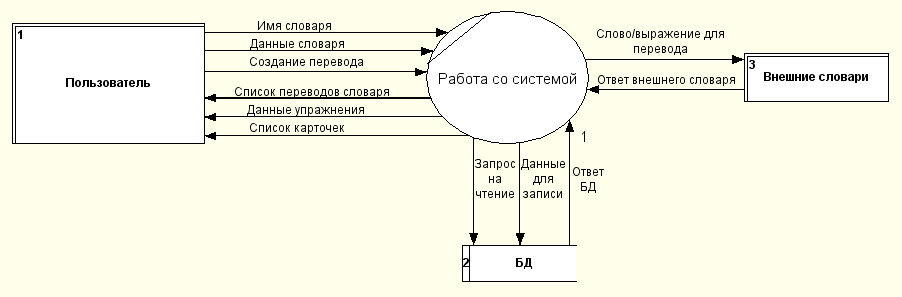
\includegraphics[width=\linewidth]{main-process}
    \caption{\code{DFD}-диаграмма основного процесса системы}
    \label{fig:main-process}
\end{figure}

На рисунке \ref{fig:translation-creation-process} изображена
\code{DFD}-диаграмма процесса создания перевода:

\begin{figure}[H]
    \centering
    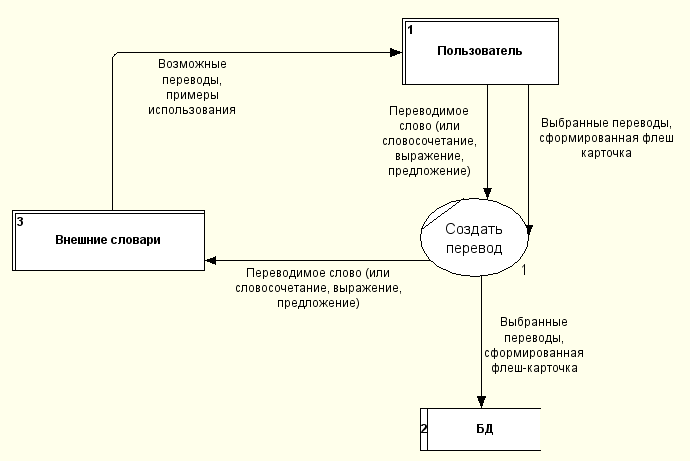
\includegraphics[width=\linewidth]{translation-creation-process}
    \caption{\code{DFD}-диаграмма процесса создания перевода}
    \label{fig:translation-creation-process}
\end{figure}

На рисунке \ref{fig:excercise-receival-process} изображена \code{DFD}-диаграмма
процесса получения упражнений:

\begin{figure}[H]
    \centering
    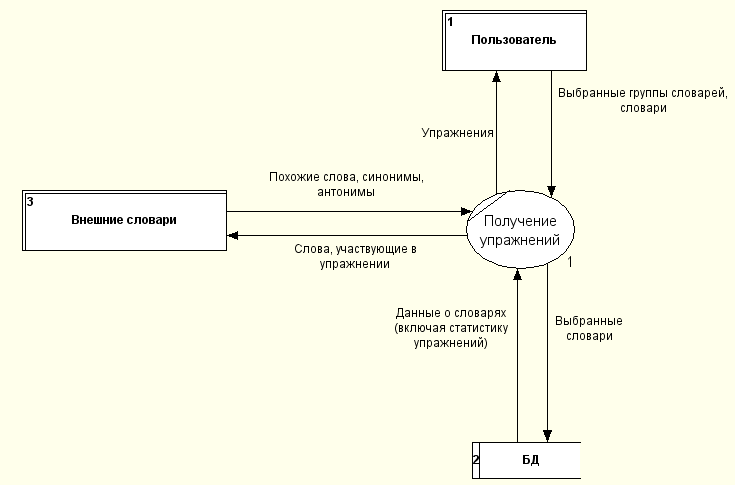
\includegraphics[width=\linewidth]{excercise-receival-process}
    \caption{\code{DFD}-диаграмма процесса получения упражнений}
    \label{fig:excercise-receival-process}
\end{figure}

\section*{Выводы}
В ходе выполнения лабораторной работы были изучены общие положения о
моделировании потоков данных и компонентов диаграммы потоков данных \code{DFD},
построены диаграммы потоков данных системы-сервиса для изучения английского
языка в системе моделирования \code{Ramus Educational}.
\end{document}